\documentclass{article}

% if you need to pass options to natbib, use, e.g.:
% \PassOptionsToPackage{numbers, compress}{natbib}
% before loading nips_2017
%
% to avoid loading the natbib package, add option nonatbib:
% \usepackage[nonatbib]{nips_2017}

\usepackage[final]{nips_2017}

% to compile a camera-ready version, add the [final] option, e.g.:
% \usepackage[final]{nips_2017}

\usepackage[utf8]{inputenc} % allow utf-8 input
\usepackage[T1]{fontenc}    % use 8-bit T1 fonts
\usepackage{hyperref}       % hyperlinks
\usepackage{url}            % simple URL typesetting
\usepackage{booktabs}       % professional-quality tables
\usepackage{amsfonts}       % blackboard math symbols
\usepackage{nicefrac}       % compact symbols for 1/2, etc.
\usepackage{microtype}      % microtypography
\usepackage{graphicx}
\hypersetup{hidelinks}
\usepackage{bm}
\usepackage{caption}
\usepackage{subcaption}
\title{Reinforcement Peer Prediction: A Reinforcement Learning Framework for Eliciting Information}

% The \author macro works with any number of authors. There are two
% commands used to separate the names and addresses of multiple
% authors: \And and \AND.
%
% Using \And between authors leaves it to LaTeX to determine where to
% break the lines. Using \AND forces a line break at that point. So,
% if LaTeX puts 3 of 4 authors names on the first line, and the last
% on the second line, try using \AND instead of \And before the third
% author name.

\author{
  Zehong Hu \\
  Nanyang Technological University\\
  \texttt{huze0004@e.ntu.edu.sg} \\
  %% examples of more authors
  \And
  Yang Liu \\
  Harvard University \\
  \texttt{yangl@seas.harvard.edu}\\
  \And
  Yitao Liang \\
  University of California, Los Angeles \\
  \texttt{yliang@cs.ucla.edu}
   \And
  Jie Zhang \\
  Nanyang Technological University \\
  \texttt{zhangj@ntu.edu.sg}
  %% Coauthor \\
  %% Affiliation \\
  %% Address \\
  %% \texttt{email} \\
  %% \AND
  %% Coauthor \\
  %% Affiliation \\
  %% Address \\
  %% \texttt{email} \\
  %% \And
  %% Coauthor \\
  %% Affiliation \\
  %% Address \\
  %% \texttt{email} \\
  %% \And
  %% Coauthor \\
  %% Affiliation \\
  %% Address \\
  %% \texttt{email} \\
}

\begin{document}
% \nipsfinalcopy is no longer used

\maketitle

\begin{abstract}
Traditional peer prediction mechanisms are designed by assuming an idealized worker model.
However, in practice, the worker model is often violated, causing the mechanisms to fail.
In this paper, we propose the first model-free reinforcement peer prediction mechanism where a data requester wants to dynamically adjust the incentive level to maximize his revenue.
To accurately estimate data requester's revenue and workers' state, we derive their posterior distributions and sample the distributions with Gibbs sampling.
Considering the inferred revenue and state are not accurate, we employ online Gaussian process regression to learn the revenue corresponding to different incentive levels and utilize the classic $\epsilon$-greedy strategy to choose the optimal incentive level.
The experiments on different worker models show that our mechanism can significantly increase data requester's revenue.
\end{abstract}

\section{Introduction}
Crowdsourcing, which elicits useful information from a crowd of online human workers, has arisen as a promising method to facilitate the development of machine learning systems.
For example, a popular application of crowdsourcing is to generate labels for large scale machine learning datasets such as RTE~\cite{snow2008cheap} and ImageNet~\cite{deng2009imagenet}.
Notwithstanding its high efficiency and immediate availability, one salient concern about crowdsourcing is the quality of collected answers, because it is often difficult or too costly to verify workers' answers.
This problem is called information elicitation without verification~\cite{waggoner2014output}.
A class of incentive mechanisms, collectively called peer prediction, has been developed to solve this problem~\cite{miller2005eliciting,jurca2009mechanisms,witkowski2012robust,witkowski2012peer,radanovic2013robust}.
In peer prediction, the payment for one worker is decided by comparing his answers with those of his peers, and the payment rules are elegantly designed so that truthful report is a game-theoretic equilibrium for all workers.


Effort elicitation is another goal considered by more recent peer prediction mechanisms~\cite{witkowski2013dwelling,dasgupta2013crowdsourced,shnayder2016informed,liu2017sequential}.
In these mechanisms, workers are incentivized not only to report truthfully, but also to generate high quality answers by exerting their maximal efforts.
For all the aforementioned peer prediction mechanisms, one essential precondition is an explicitly-known worker model which includes workers' utility function and the assumption that workers are fully rational and only take the utility-maximizing strategy.
However, in practice, workers may be bounded rational~\cite{mckelvey1995quantal,jurca2007robust}.
Or, they do not calculate the utility-maximizing strategy but gradually adjust their strategy according to the interaction with the peer prediction mechanism~\cite{chastain2014algorithms,stojic2015human}.
In some cases, workers' utility function may also be different from our anticipation~\cite{bergemann2013introduction}.
To avoid this precondition, we propose to decide the payment for workers by using reinforcement learning.
It learns the optimal payment based on workers' contributions at each step.
Nevertheless, there are two main challenges.
Firstly, classic reinforcement learning focuses on the interaction between a single agent and its environment.
It does not consider the game among workers, and thus may violate the incentive compatibility requirement that rational workers should be able to gain the maximal utility by reporting truthfully and exerting maximal efforts.
Secondly, no ground-truth answers are available for evaluating the benefits of workers.
Hence, we need to find a proper way to compute workers' contributions so that reinforcement learning can be applied.

The main contributions of this paper are the following four aspects.
Firstly, we propose the first model-free reinforcement peer prediction mechanism.
Our mechanism uses reinforcement learning to calculate the overall incentive level, traditional peer prediction mechanisms to decide the payment for each worker, and Bayesian inference to evaluate workers' contributions.
Secondly, classic Bayesian inference algorithms for crowdsourcing (e.g. the Dawid-Skene estimator~\cite{dawid1979maximum}) suffer from local optimum, causing the estimation of workers' contributions to be biased.
This bias will further mislead reinforcement learning.
Thus, we derive the explicit posterior distribution of workers' contributions and employ Gibbs sampling for inference to eliminate the bias.
Thirdly, in our mechanism, the inferred contributions are corrupted by noise and we can only observe the last step worker state rather than the current one.
Hence, in reinforcement learning, we use the online Gaussian process regression to learn the Q-function and replace the unknown current state with the couple of the last step state and incentive level.
Fourthly, we conduct empirical evaluation on different worker models, which shows that our mechanism can significantly increase the revenue of using crowdsourcing.

\section{Problem Formulation}
Suppose in our system there are one data requester and $N$ candidate workers denoted by $\mathcal{C}=\{1,\ldots, M\}$, where $M\geq 4$.
At every stage, the data requester assigns $M$ binary answer tasks, with answer space $\{1,2\}$, to workers.
At stage $t$, for task $i$, worker $j$'s label can be written as $L_{t}(i,j)$, and correspondingly our mechanism needs to pay $P_{t}(i,j)$.
Besides, we use $L_{t}(i,j)=0$ to denote that task $i$ is not assigned to worker $j$, and thus $P_{t}(i,j)=0$.
After collecting labels, the data requester will aggregate labels via Bayesian inference~\cite{zheng2017truth}, and the label accuracy can be written as $A_t$.
Thus, the revenue of the data requester at stage $t$ can be calculated as:
\begin{equation}
r_t = F(A_t) - \eta {\sum}_{i=1}^{N}{\sum}_{j=1}^{M}P_{ij}
\end{equation}
where $F(\cdot)$ maps accuracy into revenue. In practice, the higher accuracy, the better. Meanwhile, the collected labels can only be used when their accuracy reaches a certain requirement.
Thus, we set $F(A_t)=A^{n}_t$ in this paper.
It is worth noting that our reinforcement peer prediction mechanism does not require any specific formulation of the $F$ function.
Suppose our mechanism goes for $T$ stages.
Thus, the goal of our mechanism is to maximize the accumulative revenue, namely $R = \sum_{t=1}^{T} r_t$.

\section{Reinforcement Peer Prediction}
\begin{figure}[htb]
        \centering
        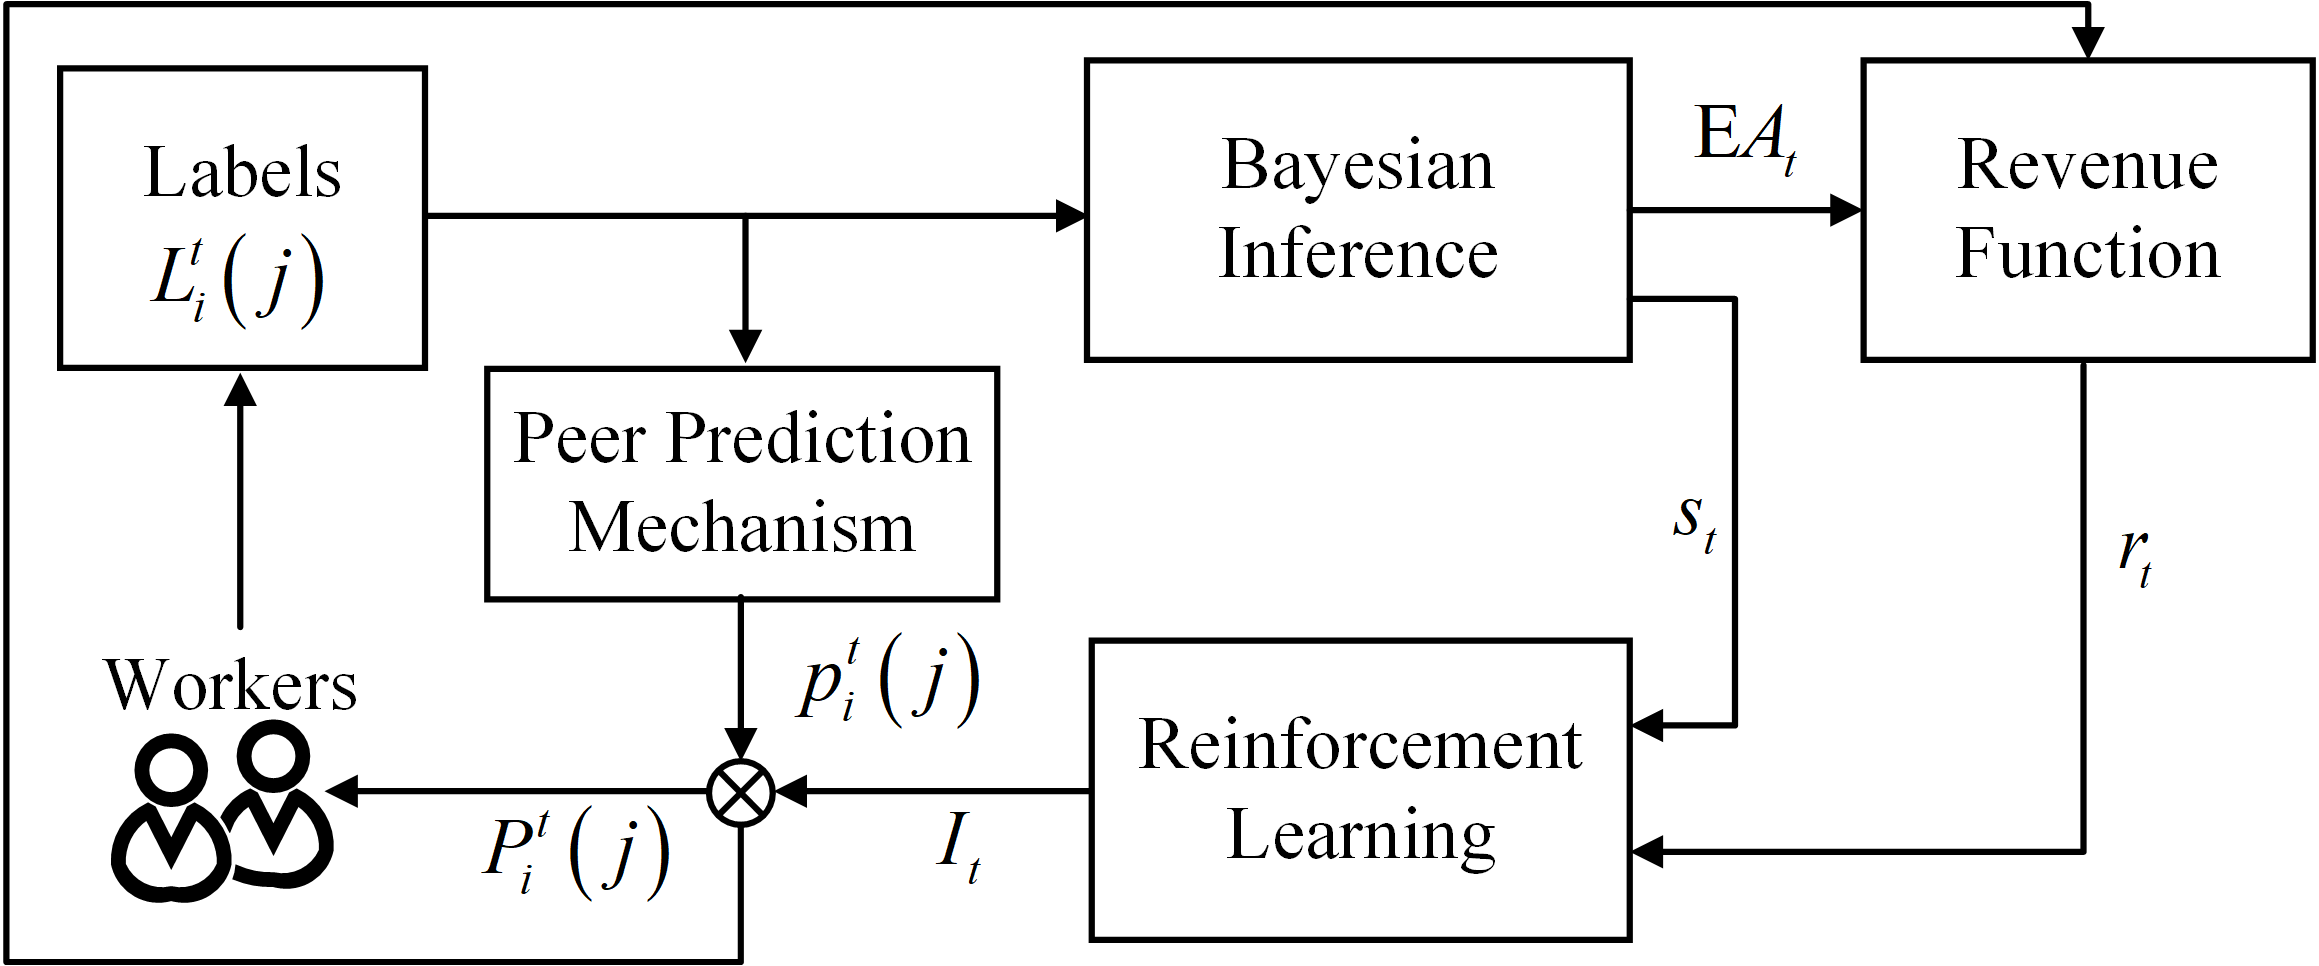
\includegraphics[width=0.6\textwidth]{image/Mechanism}
        \caption{\label{ED1} The architecture of our reinforcement peer prediction mechanism}
\end{figure}
We present the architecture of our mechanism in Figure~\ref{ED1}. At step $t$, our mechanism decides the payment for workers as $P_{t}(i,j)=I_t \cdot p_{t}(i,j)$, where $I_t$ denotes the incentive level calculated by our reinforcement learning algorithm.
$p_t(i,j)$ denotes the output of the peer prediction mechanism.
By doing so, we can ensure the reinforcement learning does not break the incentive compatibility requirement, that is, truthful report and exerting maximal efforts is always a Nash equilibrium for all workers.
Besides, we use Bayesian inference to aggregate the collected labels.
Since the ground-truth answers are unavailable, we cannot directly calculate the accuracy $A_t$.
Thus, we use the expected accuracy $\mathbb{E}A_t$ instead.
It can be calculated as $\mathbb{E}A_t = \frac{1}{N}\sum_{i=1}^{N} \textrm{Pr}(L_i = y_i)$, where $L_i$ and $y_i$ denote the aggregated and true label, respectively.
Meanwhile, Bayesian inference can also output the confusion matrices of all workers and the distribution of task labels $\left[\textrm{Pr}(l=1), \textrm{Pr}(l=2)\right]$.
For worker $j$, his confusion matrix $C_j = [c_{jkg}]_{2\times 2}$, where $c_{jkg}$ denotes the probability that worker $j$ labels a task in class $k$ as class $g$.
Since the accuracy of labels are determined by the overall quality of workers, how an individual worker performs is not the concern of our reinforcement learning algorithm.
Thus, we denote the state of the whole worker crowd $s_t$ by workers' average probability of being correct, namely $s_t = \sum_{k\in\{1,2\}}\textrm{Pr}(l=k)\cdot \frac{1}{M}\sum_{j=1}^{M}c_{jkk}$.
After workers receive the payment, they may adjust their strategies, which will lead to the change $s_t$.
However, when computing the incentive level $I_{t+1}$, we only has the last step state $s_t$.
In other words, the state observation has one-stage delay, which makes our reinforcement learning problem different from traditional ones.

\noindent \textbf{Peer Prediction Mechanism:} We adopt the state-of-the-art mechanism proposed by \cite{dasgupta2013crowdsourced}.  For each task-worker pair $(i, j)$, it selects a reference worker $k$. Suppose workers $j$ and $k$ have been assigned $d$ other distinct tasks $\{j_1,\ldots,j_d\}$ and $\{k_1,\ldots, k_d\}$, respectively. Then, the payment $p_t(i,j)= 1[L(i,j)=L(i,k)]- \xi_{j}^d\cdot \xi_{k}^d -\bar{\xi}_{j}^d\cdot \bar{\xi}_{k}^d$, where $\xi_{k}^{d}=\sum_{g=1}^{d}1(L(i_g, k)=1)/d$ and $\bar{\xi}_{k}^{d}=1-\xi_{k}^{d}$.

\noindent \textbf{Bayesian Inference:} Suppose the prior distributions that $c_{jk1}\sim \textrm{Beta}(\alpha^{0}_{jk1},\alpha^{0}_{jk2})$ and $\textrm{Pr}(l=1)\sim \textrm{Beta}(\beta^{0}_{1},\beta^{0}_{2})$. Then, we can explicitly derive the posterior distribution of true labels as
\begin{equation}
\label{PostDist}
P(\bm{y}|\bm{L})\propto B(\bm{\beta}){\prod}_{j=1}^{M}{\prod}_{k=1}^{K} B(\bm{\alpha}_{jk})\;,\; \alpha_{jkg}={\sum}_{i=1}^{N}\delta_{ijg}\xi_{ik}+\alpha^{0}_{jkg}, \beta_k={\sum}_{i=1}^{N}\xi_{ik}+\beta^{0}_{k}
\end{equation}
where $B(\cdot)$ denotes the beta function, $\delta_{ijg}=1(L(i,j)=g)$ and $\xi_{ik}= 1(y_i=k)$. According to Gibbs sampling, we can generate posterior samples via iteratively sampling $P(y_i|\bm{L}, \bm{y}_{j\neq i})$.

\noindent \textbf{Reinforcement Learning:} When calculating the incentive level $I_{t}$ for stage $t$, the current state $s_{t}$ cannot be observed. Thus, we define our incentive policy as $\pi(I_{t}|x_t)$, where $x_t=\langle s_{t-1}, I_{t-1}, t \rangle$.
Then, the Q-function of our policy can be calculated as $Q(x_t, I_t)= \sum_{i=0}^{T-t} \gamma^{i} r_{t+i}$, where the discount factor $\gamma$ is slightly smaller than $1$ and $Q(x_{T+1}, I_{T+1})=0$.
Both the state $s_t$ and reward $r_t$ are not accurately observed.
Thus, we apply Gaussian process regression for the Q-function:
\begin{equation}
\label{GaussPro}
Q(x_t, I_t) - \gamma Q(x_{t+1}, I_{t+1}) = r_t + N(x_t,x_{t+1})
\end{equation}
where the residual $N(x_t,x_{t+1})$ is assumed to be a Gaussian process. By applying the online Gaussian process regression algorithm~\cite{engel2005reinforcement}, we can learn the Q-function. Then, we decide the incentive level $I_t$ for stage $t$ as $\arg\max Q(x_t, I_t)$ with probability $1-\epsilon$ and a random value with probability $\epsilon$.

\section{Experiments}
\begin{figure}[htb]
    \centering
    \begin{subfigure}[t]{0.32\textwidth}
        \centering
        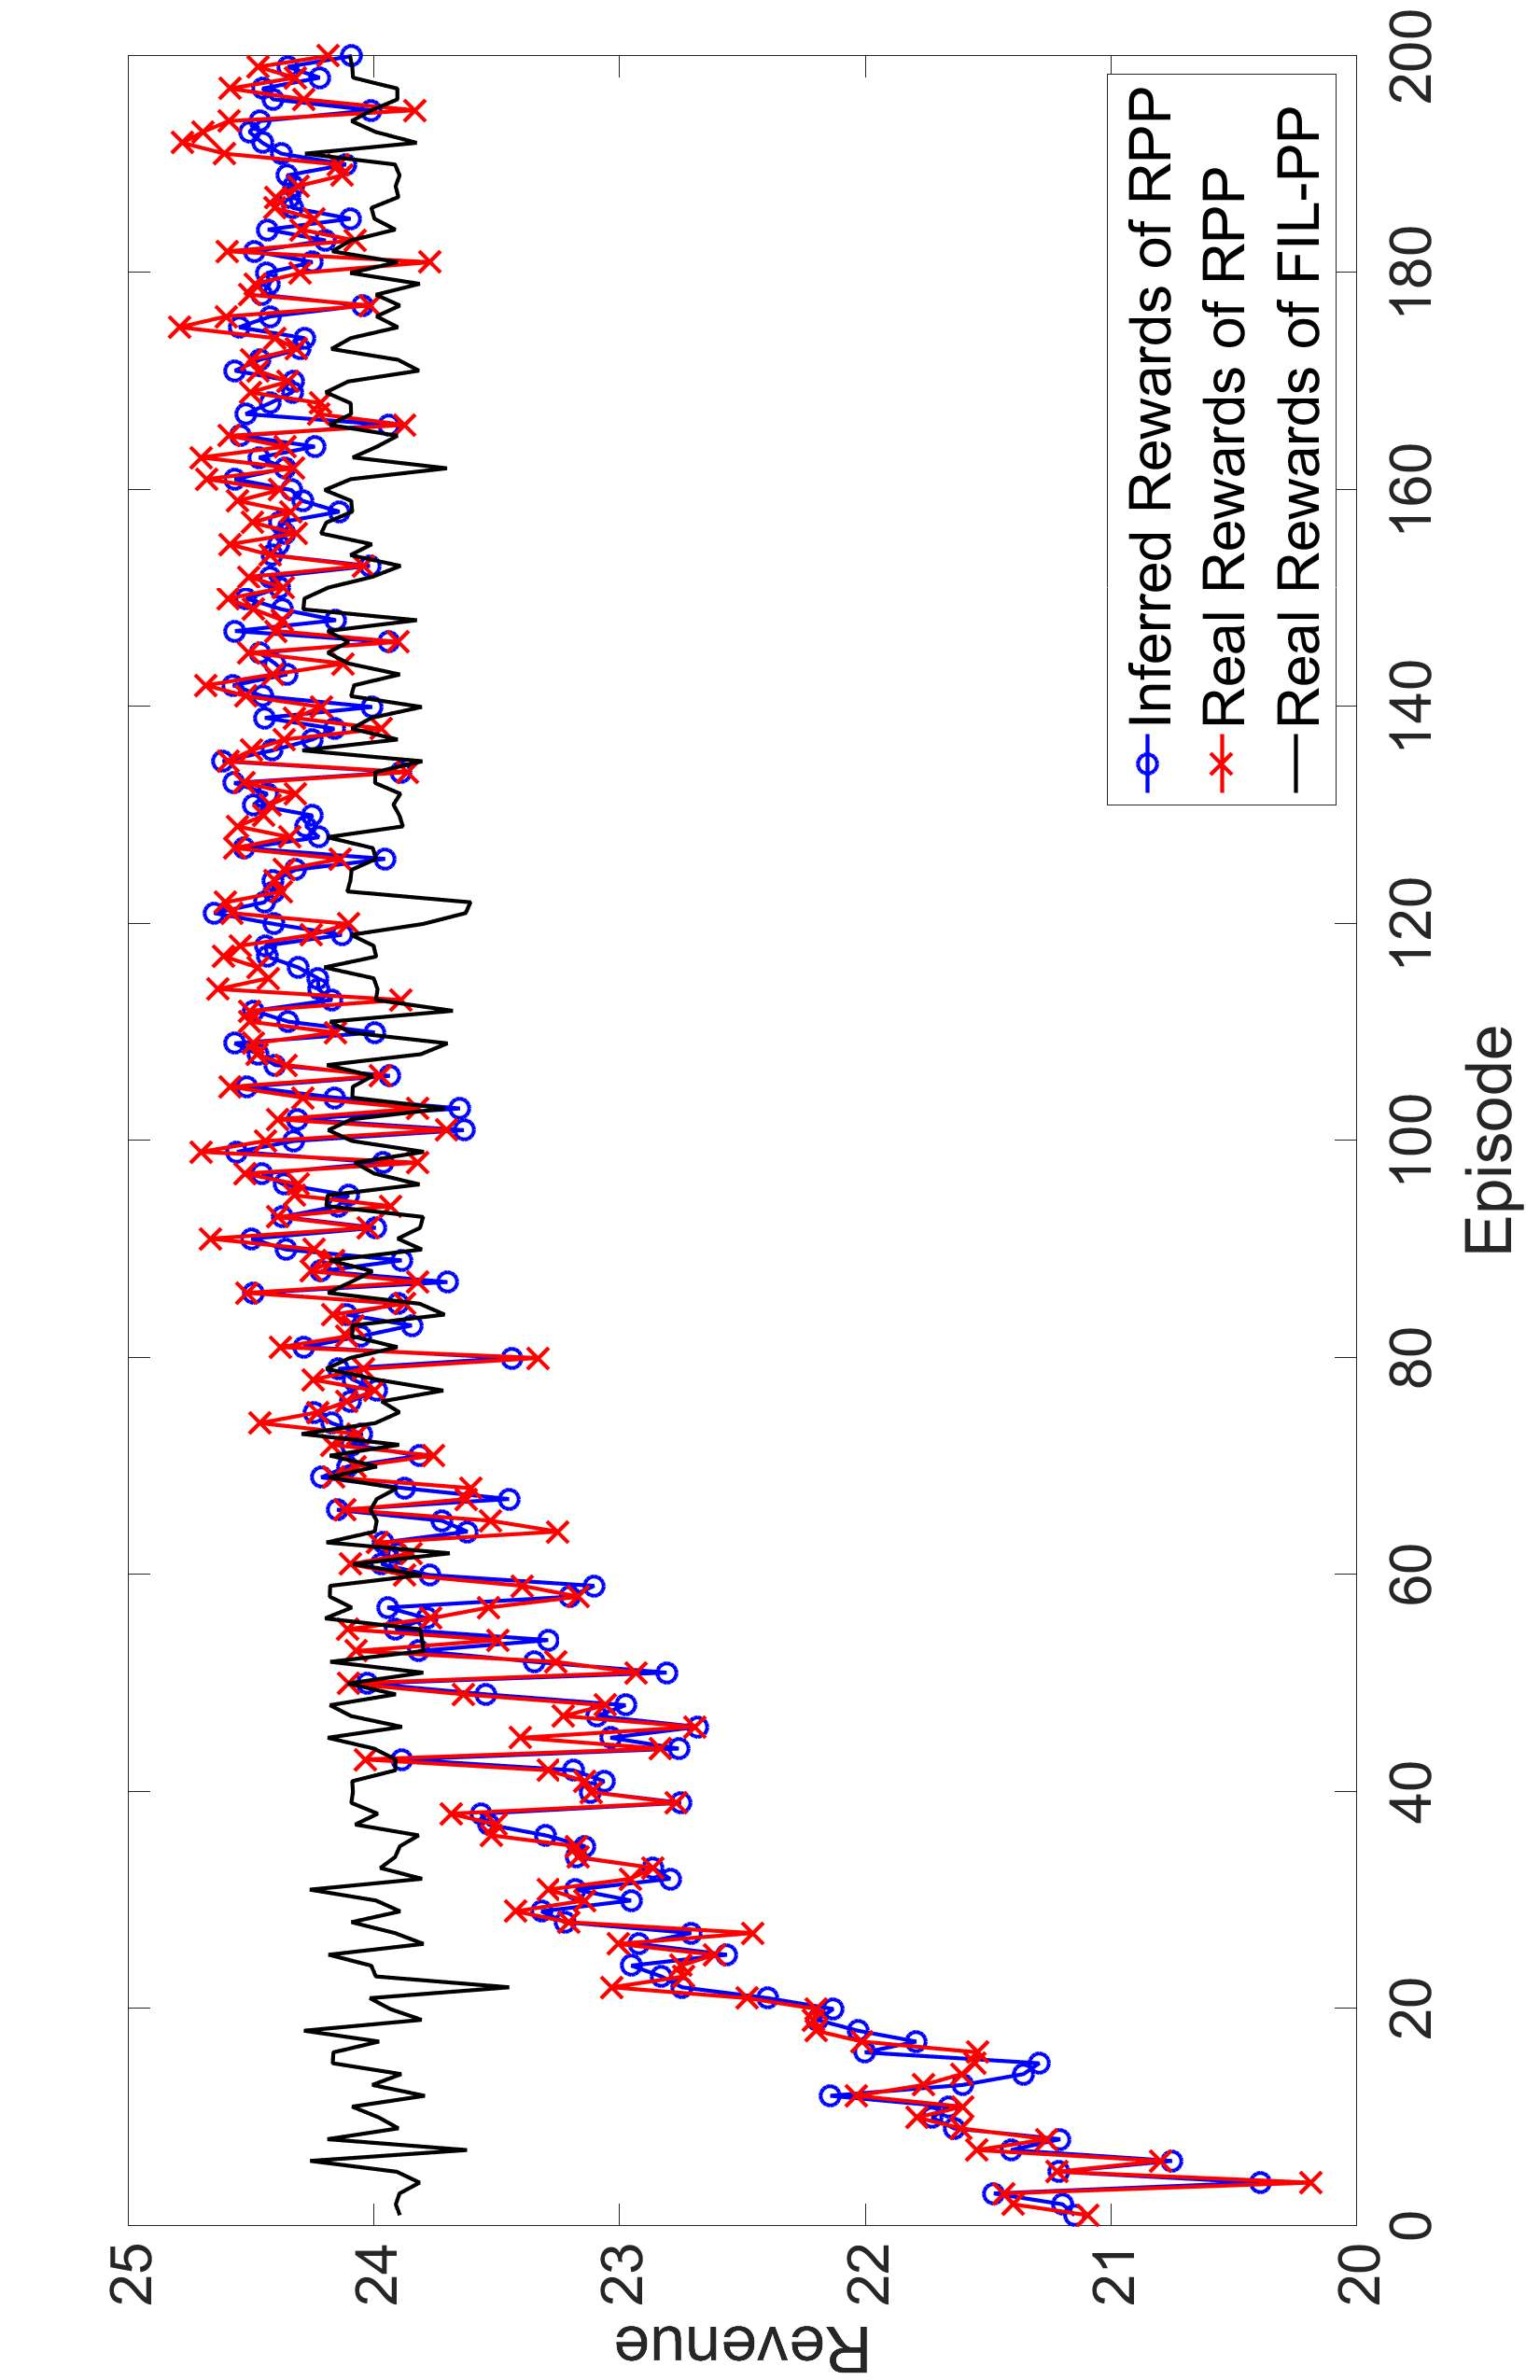
\includegraphics[width=\textwidth]{image/1}
        \caption{\label{E1} Rational Workers}
    \end{subfigure}%
    ~
    \begin{subfigure}[t]{0.32\textwidth}
        \centering
        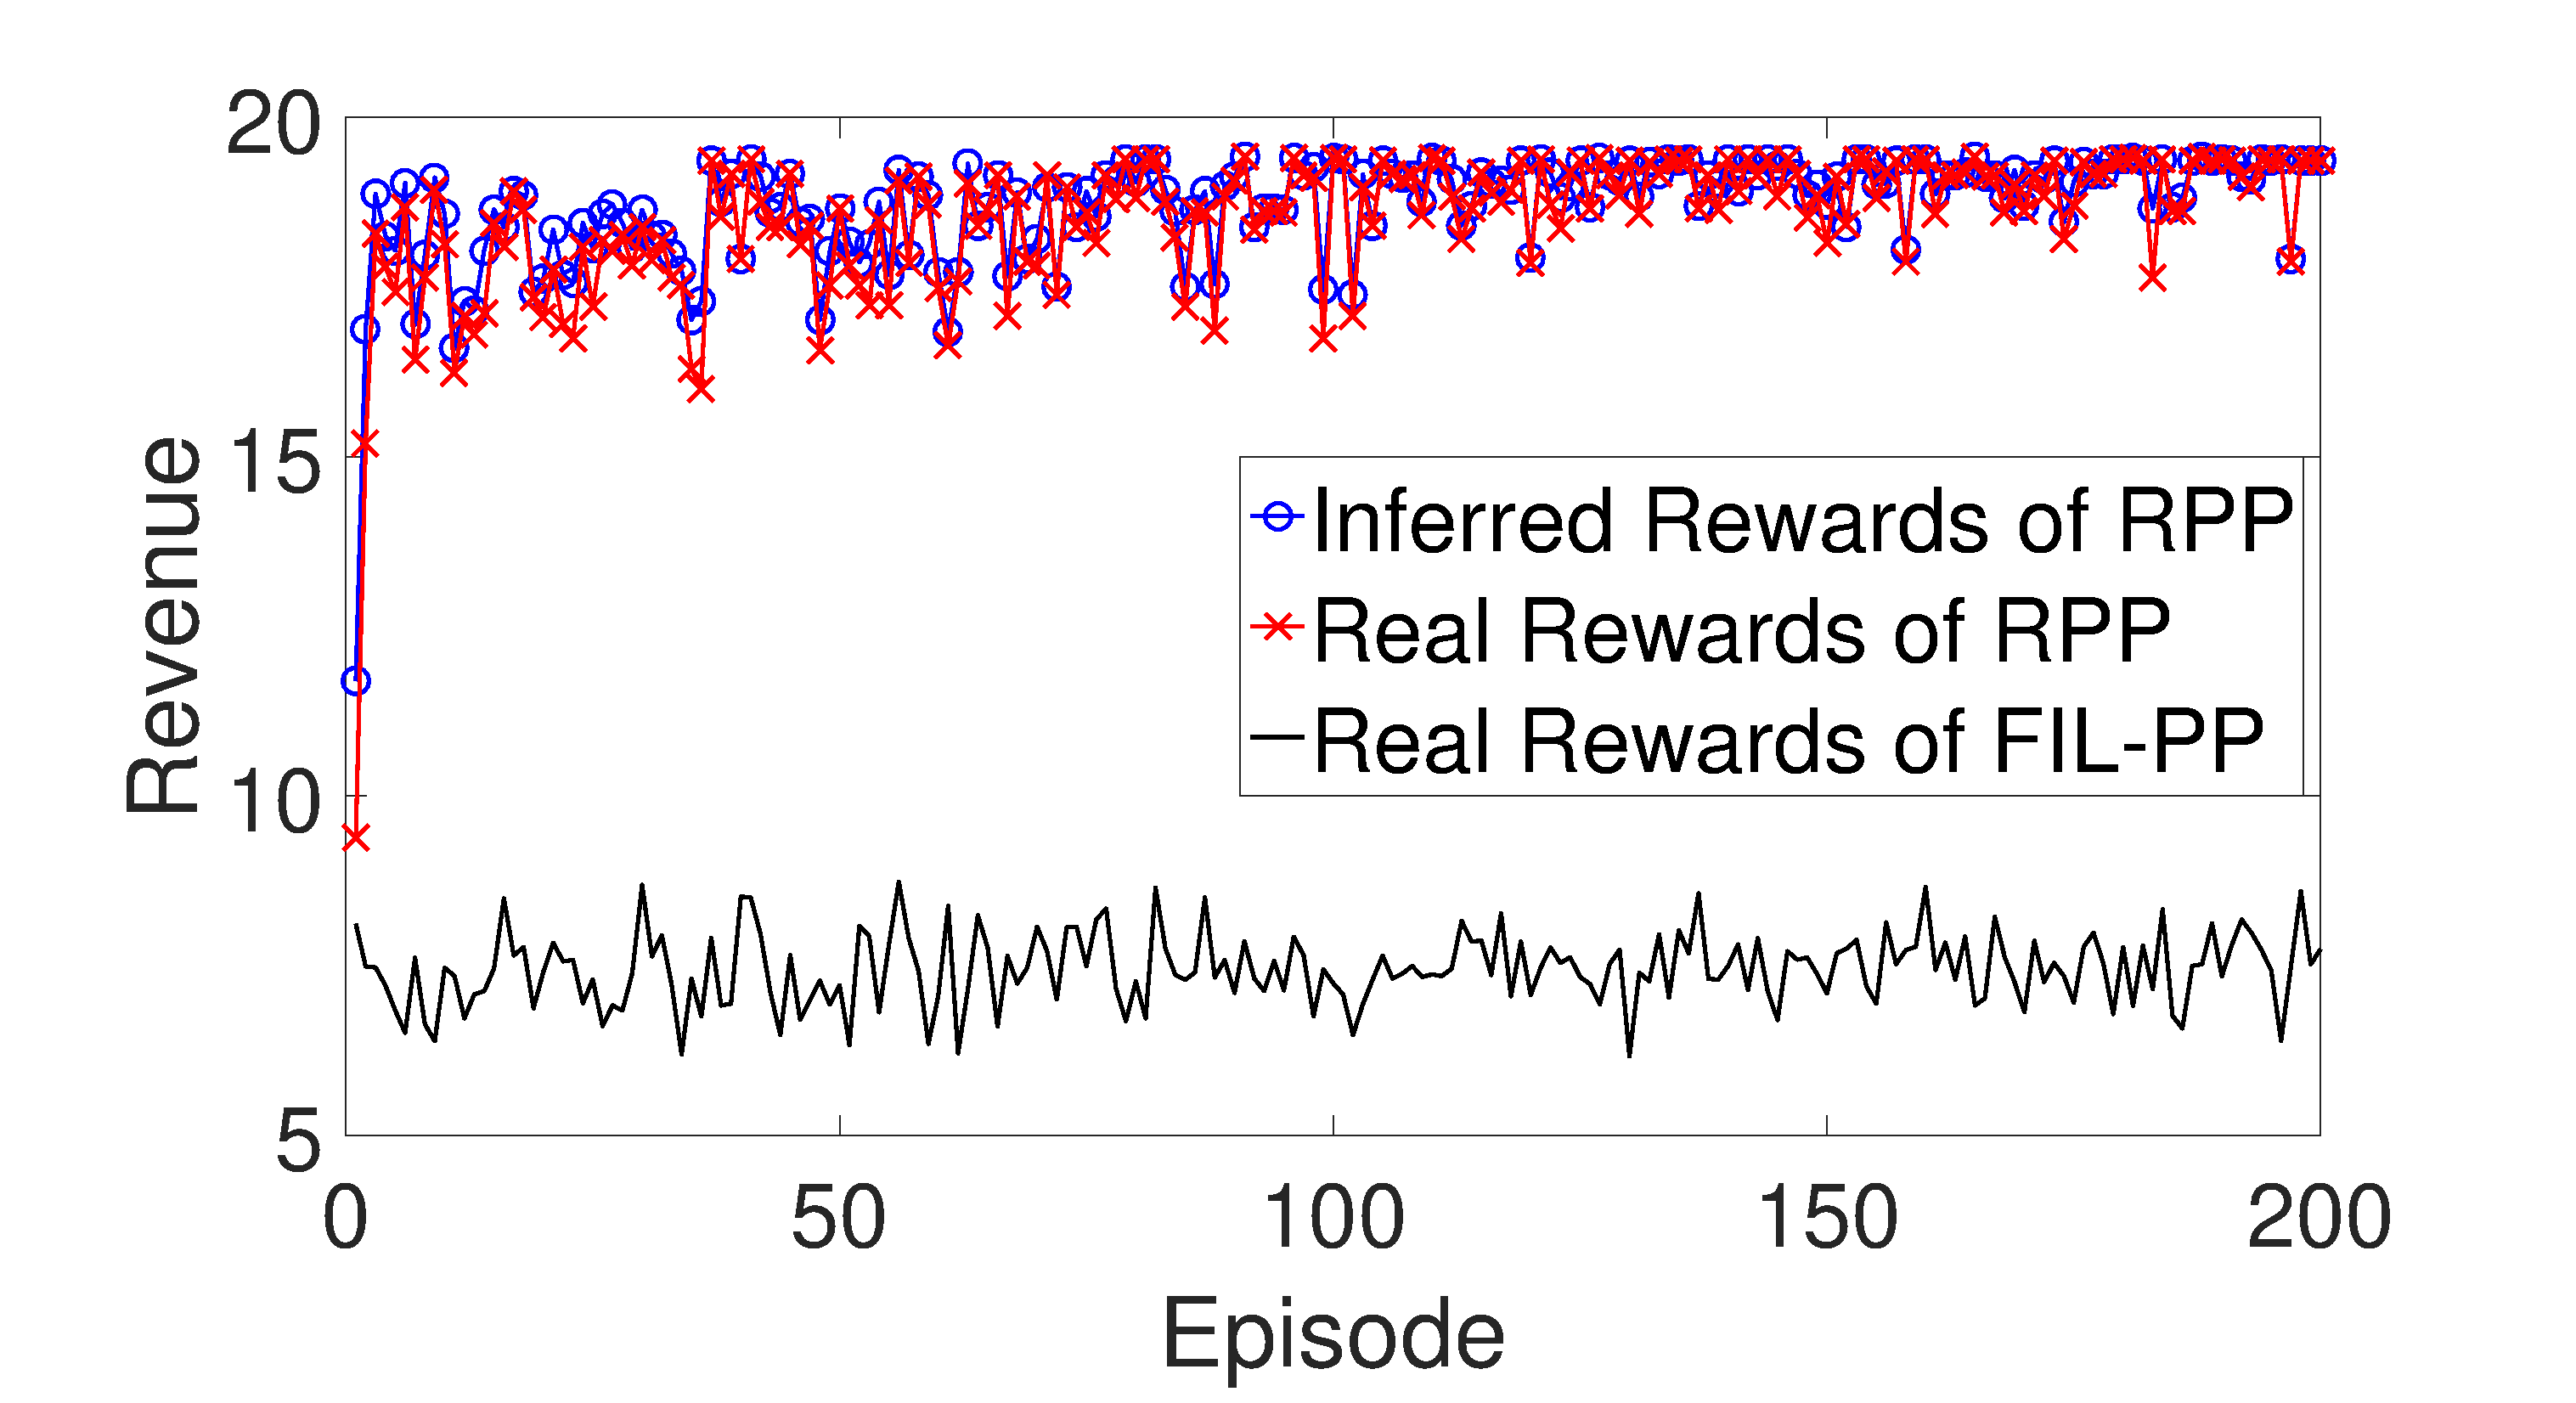
\includegraphics[width=\textwidth]{image/2}
        \caption{\label{E2}  Quantal Response Workers}
    \end{subfigure}
    ~
    \begin{subfigure}[t]{0.32\textwidth}
        \centering
        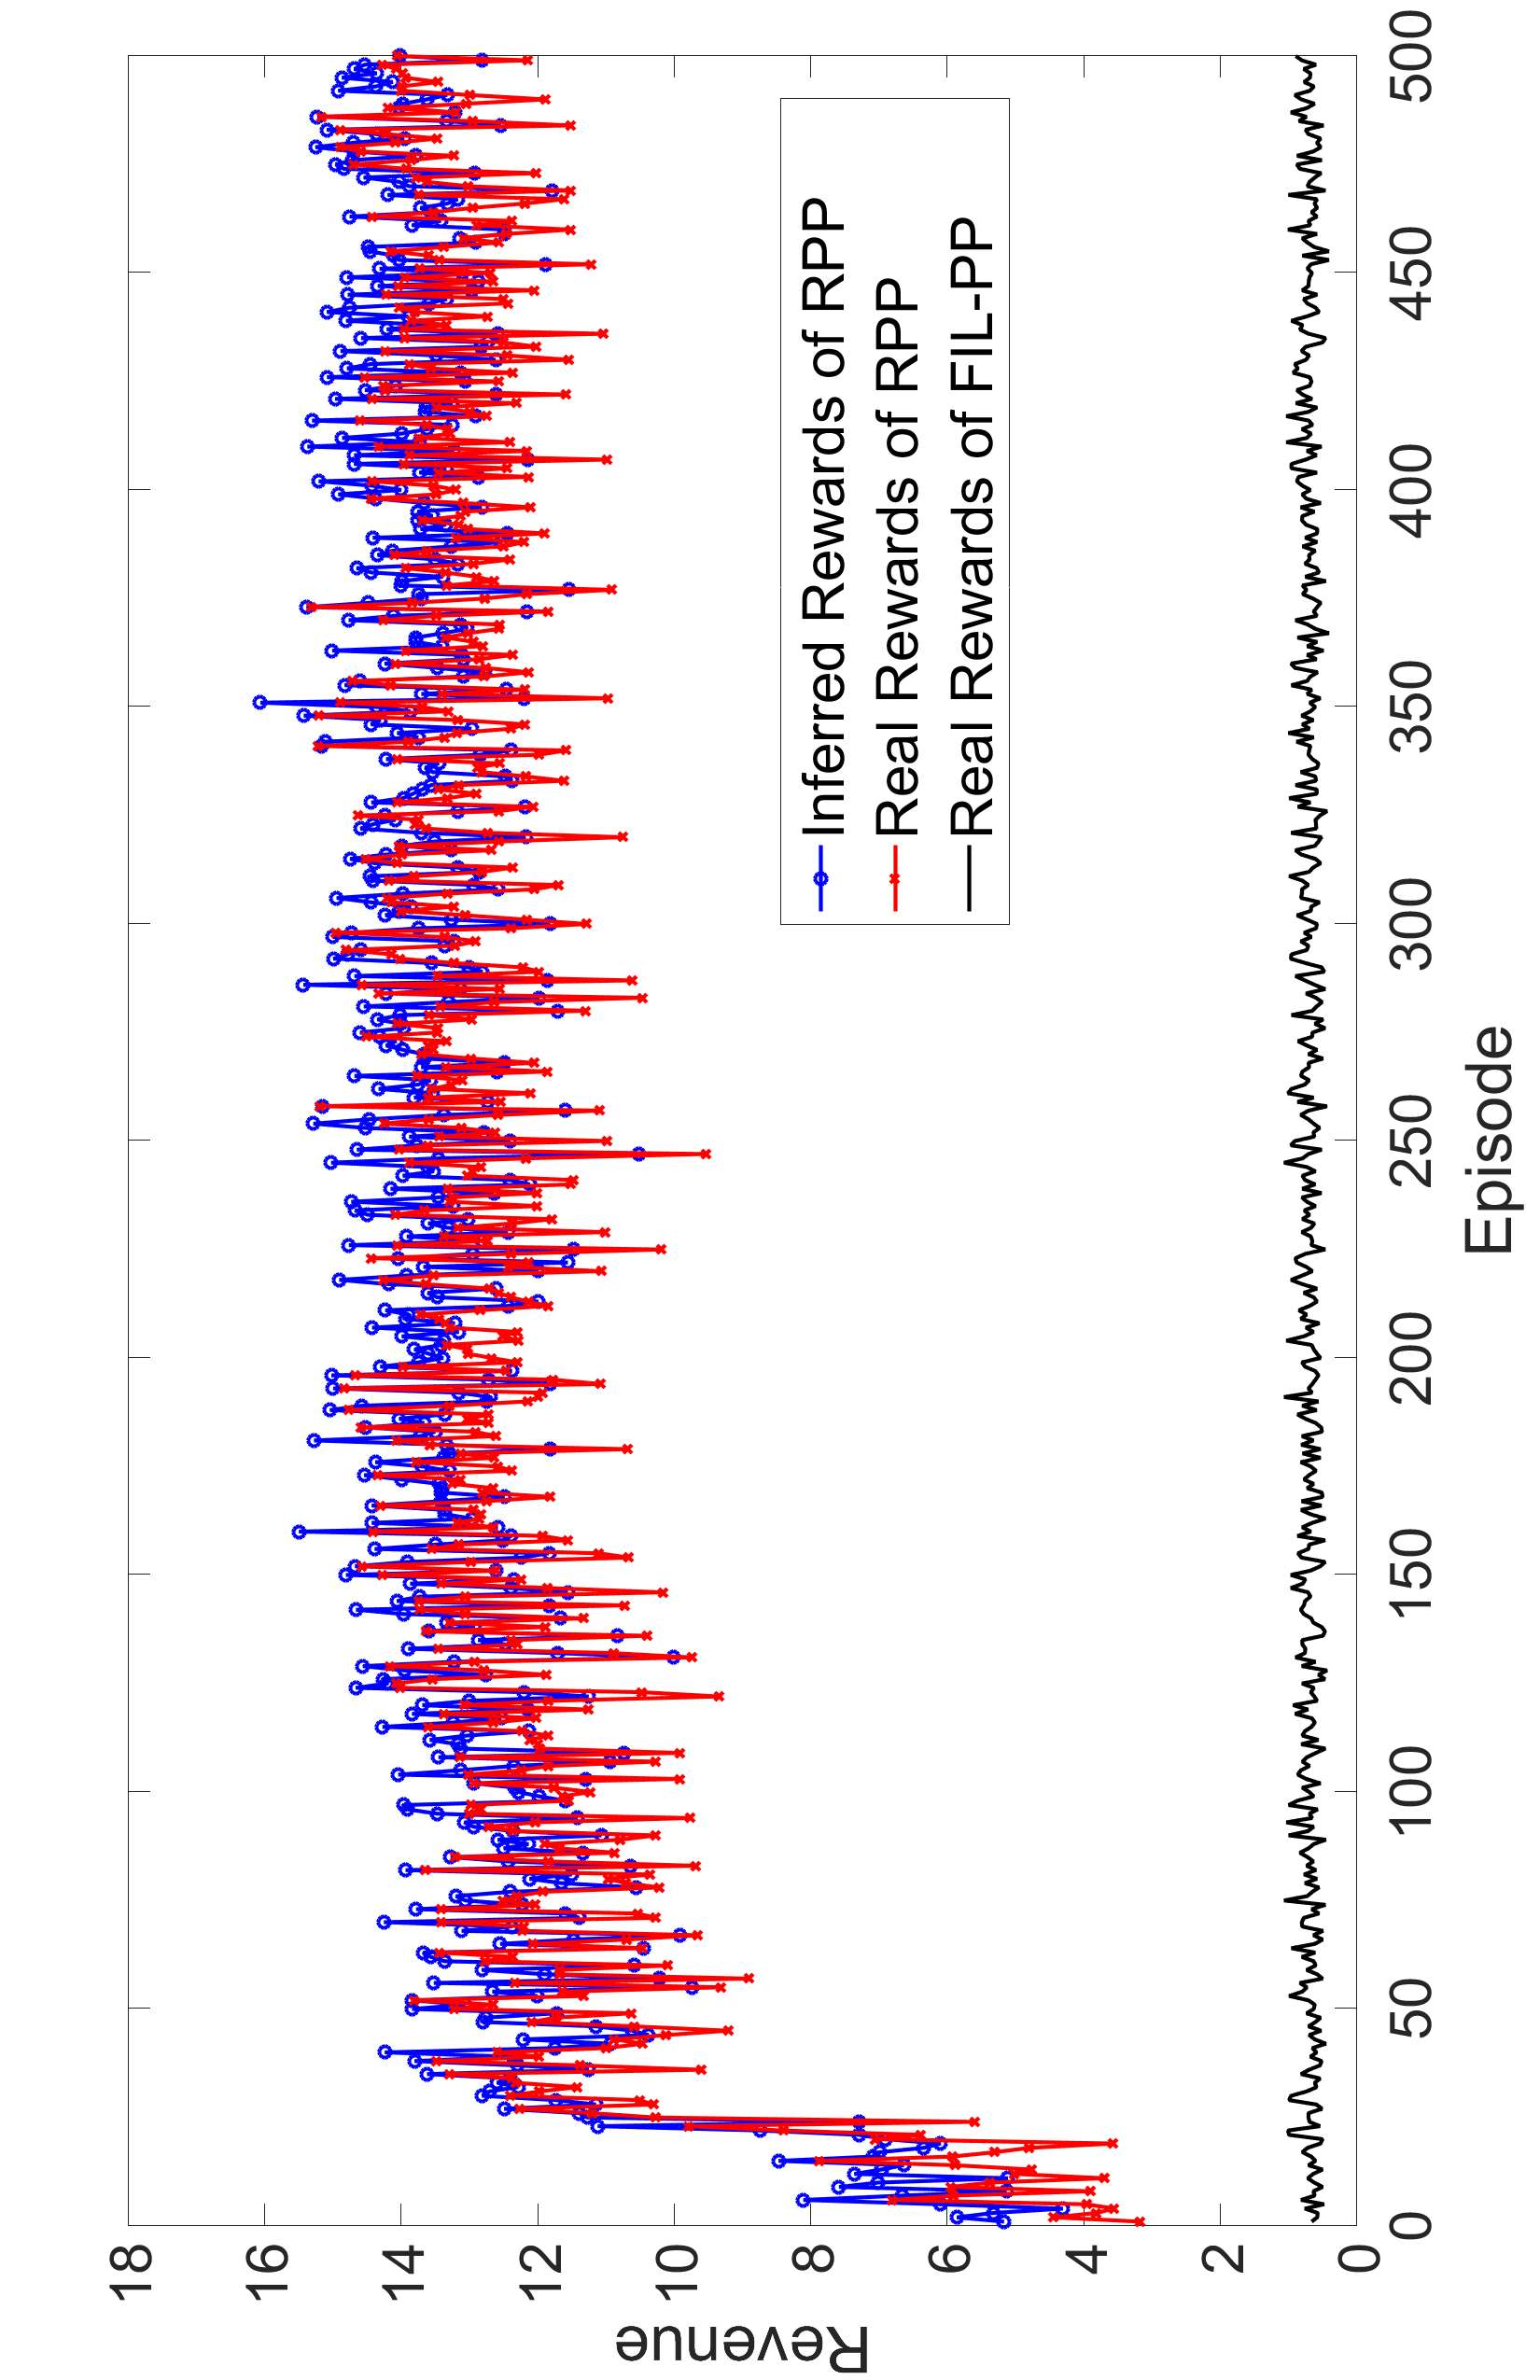
\includegraphics[width=\textwidth]{image/3}
        \caption{\label{E3}  MWUA Workers}
    \end{subfigure}    
    \caption{\label{ED}Experiments on different worker models}
    \vspace{-1mm}
\end{figure}
In Figure~\ref{ED}, we present the simulation results on different worker models.
In our experiments, we assume there are four incentive levels, namely $I_t\in \{0.1, 1.0, 5.0, 10.0\}$.
Meanwhile, we set the number of workers and tasks at each stage as $10$ and $100$, respectively.
For rational workers, we assume all workers report the true labels with probability $0.9$ for all incentive levels.
For quantal response workers, we assume workers use the quantal response model~\cite{mckelvey1995quantal} to decide whether to exert the maximal efforts.
For MWUA workers, we assume workers follow the MWUA model~\cite{chastain2014algorithms}.
From all the experiments, we can find that our reinforcement peer prediction mechanism can gradually lean the optimal incentive strategy, which significantly increase the revenue when workers are not rational.

%\subsubsection*{Acknowledgments}

%Use unnumbered third level headings for the acknowledgments. All
%acknowledgments go at the end of the paper. Do not include
%acknowledgments in the anonymized submission, only in the final paper.

\newpage
\bibliographystyle{abbrv}
\bibliography{ref}

\end{document}
